\clearpage 
\section*{\underline{Extended Data}}

%\renewcommand\thefigure{\thesection.\arabic{figure}}    
\setcounter{figure}{0}    

\begin{figure}[h!]
	\centering
	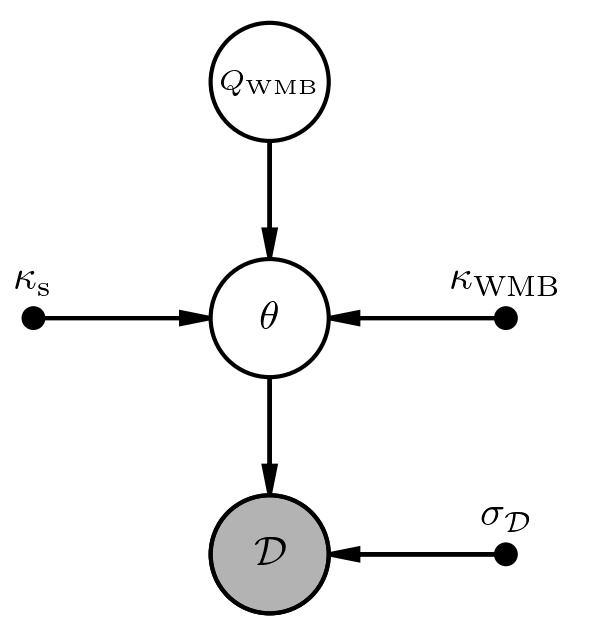
\includegraphics[width=0.6 \textwidth]{pgm_models.jpg}
	\caption{\textbf{A probabilistic graphical model (PGM) represented algebraically in Equation \ref{eq:modelll}.} The shaded circle indicates observed data, and solid black points represent other fixed information, such as the KDEs and observational uncertainties. The remaining circles represent parameters. The underline indicates that the symbol represents a set of parameters or data. Here, $\kappa_{\rm{s}}$ and $\kappa_{\rm WMB}$ represent the KDEs of standard and WMB model populations respectively. $Q_{\rm{WMB}}$ is the mixture model weighting factor. The latent parameters $\theta$, our observations $\mathcal{D}$ and their uncertainties $\sigma_{\mathcal{D}}$ include temperature (\teff), mass ($M$), log-age ($\ln(t)$), metallicity (\feh) and log-rotation ($\ln(P)$). This model is \textit{hierarchical}, as all the latent parameters are drawn from the common probability distribution set by $Q_{\rm{WMB}}$ and described in Equation \ref{eq:mixturell}.}
	\label{fig:pgm}
\end{figure}
 